\section{Programas}
\label{sec:programas}

\begin{table}[H]
    \centering
    \label{tab:programas}
    \begin{tabular}{|c|c|}
        \hline Pão Caseiro & Pão Rústico \\ \hline
        \begin{tabular}{c|c}
            Fase da Fabricação & Tempo (segundos) \\
            Amassar & 10 \\
            Levedar & 4 \\
            Cozer & 10 \\
        \end{tabular}
        &
        \begin{tabular}{c|c}
            Fase da Fabricação & Tempo (segundos) \\
            Amassar & 15 \\
            Levedar & 8 \\
            Cozer & 10 \\
        \end{tabular} \\ \hline
    \end{tabular}
    \caption{Programas de Pão}
\end{table}

\section{Funcionamento}
\label{sec:funcionamento}

A máquina inicializa permitindo o utilizador selecionar o programa a ser executado.\ Para tal, deve colocar o interruptor `Selecionador Programa' na posição do programa que deseja.\ O `Pão Caseiro' será a posição inicial do interruptor e o `Pão Rústico' será a outra posição.\ Sempre que a máquina é reiniciada estas posições são reatribuídas.\ Os programas, bem como as suas durações, são descritos em cima: Tabela~\ref{tab:programas}.

O utilizador pode também escolher o atraso inicial a ser aplicado e, para isso, terá de usar os 7 interruptores do `Selecionador Atraso' para indicar o número, este terá de ser introduzido em binário e a máquina irá converter para decimal.\ Este valor poderá variar entre 0 e 90 segundos e qualquer valor superior a isso será interpretado como 90.

Após a seleção do programa e do atraso inicial o utilizador poderá clicar no botão `Start/Stop' para iniciar a máquina.\ O programa irá começar assim que o atraso inicial chegar a 0.\ Poderá ver a fase em que o programa se encontra com os `LEDS Display Fase':
\begin{itemize}
    \item 3 LEDS ligados $\rightarrow$ Amassar
    \item 2 LEDS ligados $\rightarrow$ Levedar
    \item 1 LED ligado~~~~$\rightarrow$ Cozer ou Tempo Extra
    \item 0 LEDS ligados $\rightarrow$ Standby, Atraso Inicial ou Espera da Confirmação do Tempo Extra/Reinicialização
\end{itemize}

O tempo, tanto do atraso como da programação normal poderá ser pausado e continuado em qualquer momento ao longo da sua execução.

Após o final da programação normal o utilizador terá a possibilidade de adicionar tempo extra utilizando o botão `Tempo Extra'.\ Para iniciar o mesmo, o utilizador deverá clicar no botão `Start/Stop'.\ Tal como o atraso inicial e o tempo do programa, o tempo extra também poderá ser pausado e continuado em qualquer momento.\ Se o botão de `Start/Stop' for pressionado com o tempo extra a 0 então a máquina irá ser reiniciada.\ O utilizador pode usar o tempo extra o número de vezes que desejar.

O `LED Display Execução' estará ligado durante a execução do programa normal e do tempo extra.

A máquina poderá também ser reinicada em qualquer momento usando o botão `Reset'.

\section{Esquema da Máquina}
\label{sec:esquema-da-maquina}

\begin{figure}[H]
    \center
    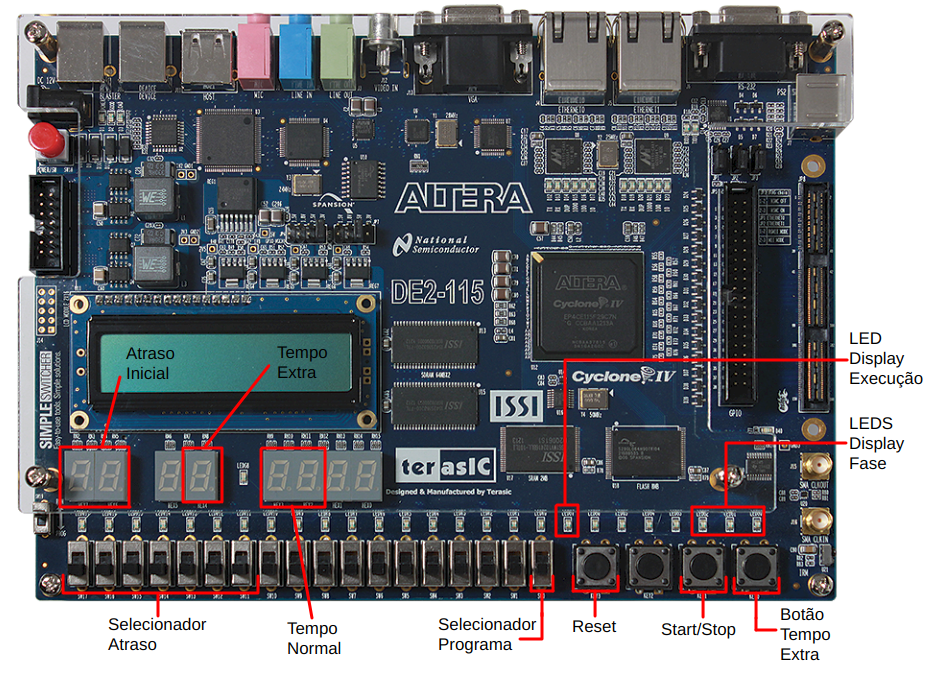
\includegraphics[scale=.4]{../images/esquema-placa}\caption{Ilustração do Esquema da Máquina}
    \label{fig:esquema-placa}
\end{figure}

\begin{itemize}
    \item \textbf{Display: Atraso Inicial} $\rightarrow$ Display para mostrar o tempo que irá decorrer antes do início da execução do programa.
    \item \textbf{Display: Tempo Extra} $\rightarrow$ Display para mostrar o tempo extra do programa.
    \item \textbf{Display: Tempo Programa} $\rightarrow$ Display para mostrar o tempo de execução do programa.
    \item \textbf{LED: Display Execução} $\rightarrow$ LED para indicar que o programa está a ser executado.
    \item \textbf{LEDS: Display Fases} $\rightarrow$ LEDS para indicar a fase do programa que está a ser executada.
    \item \textbf{Switch: Selecionador Atraso} $\rightarrow$ Série de interruptores para selecionar o tempo de atraso inicial.
    \item \textbf{Switch: Selecionador Programa} $\rightarrow$ Interruptor para selecionar o programa a ser executado.
    \item \textbf{Botão: Reset} $\rightarrow$ Botão para reiniciar a máquina.
    \item \textbf{Botão: `Start/Stop'} $\rightarrow$ Botão para iniciar ou parar a execução do programa.
    \item \textbf{Botão: Tempo Extra} $\rightarrow$ Botão para adicionar tempo extra ao programa.
\end{itemize}